\begin{figure}[h]
    \centering
    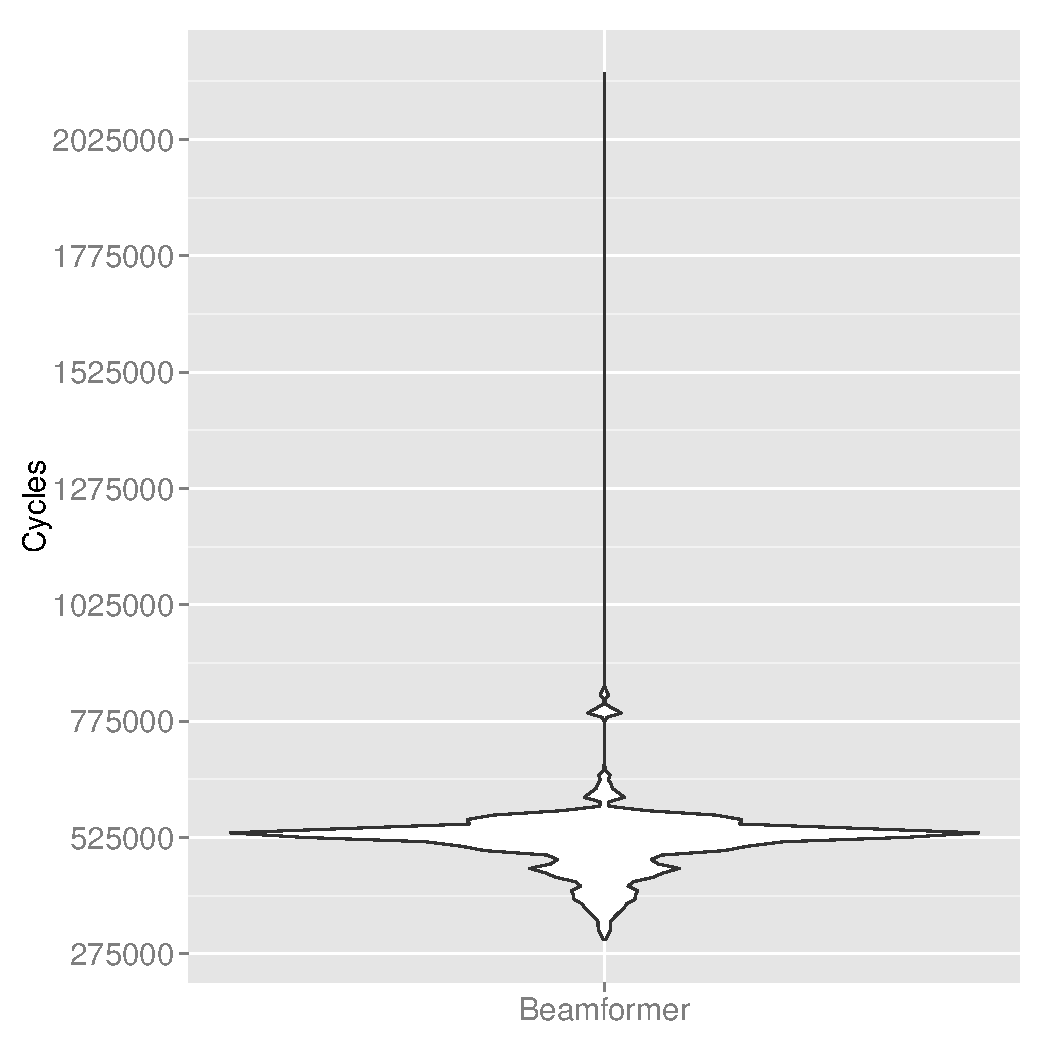
\includegraphics[width=0.7\textwidth]{streamit-paper/graphics/beamformer_motivation.pdf}
    \caption{Distribution of the runtime for Beamformer resulting from an exhaustively exploration of the hardware/software co-design space.
     The application has been partitioned into different number of threads and core compositions.}
     \label{fig:beamformermotiv}
\end{figure}

\begin{figure}[h]
    \centering
    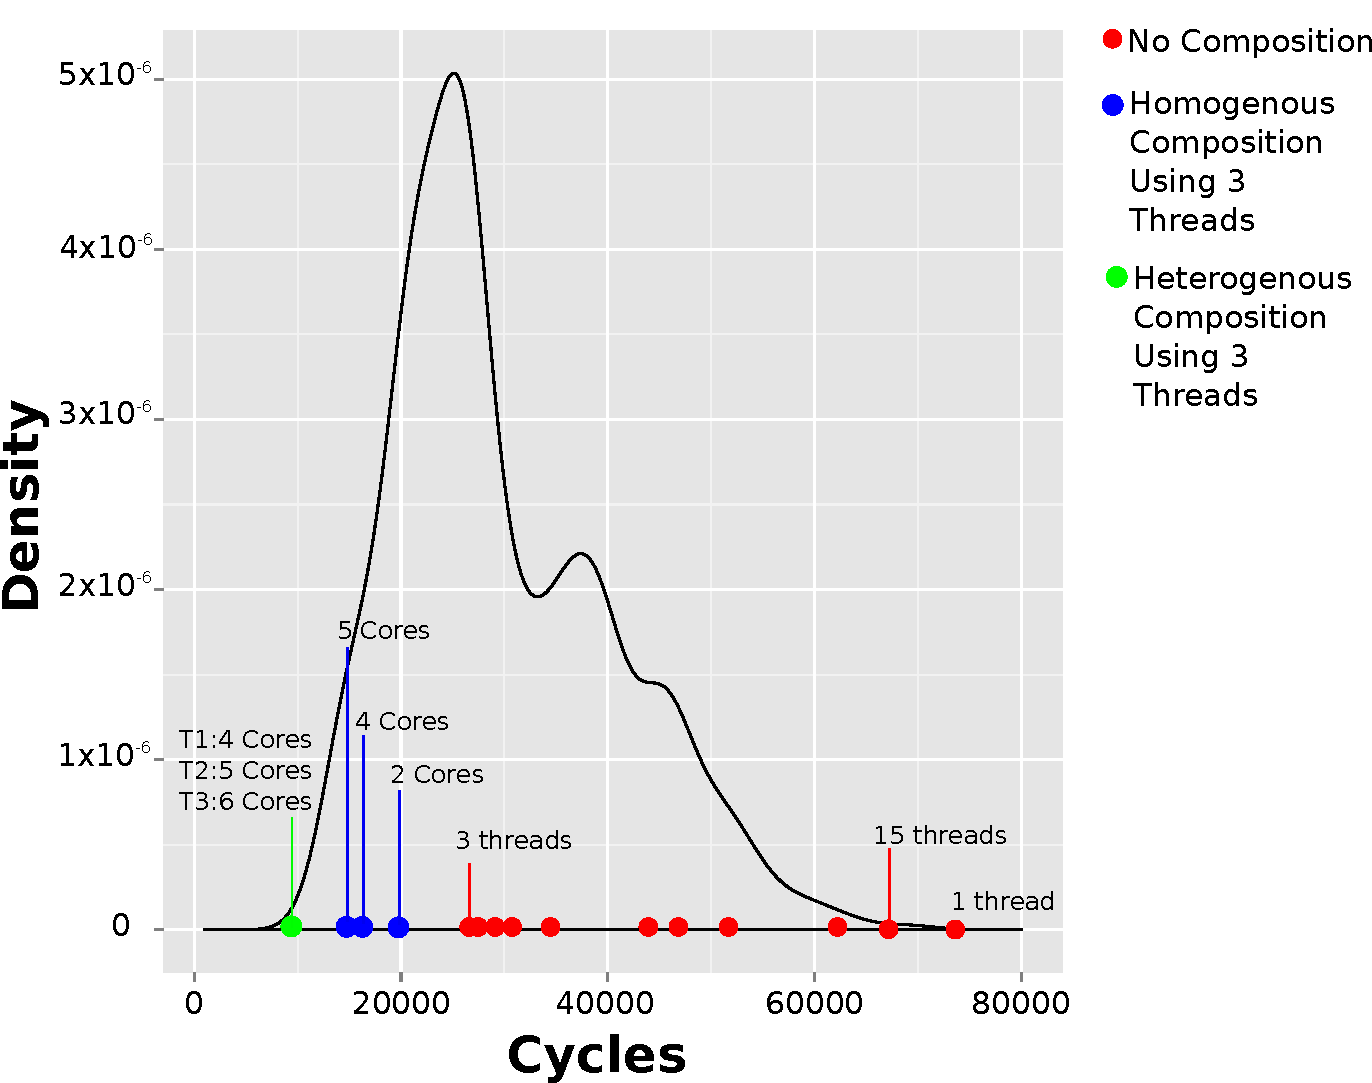
\includegraphics[width=1\textwidth]{streamit-paper/graphics/temp_motivation_2.pdf}
    \caption{Distribution of the runtime with different core composition thread pairings.}
     \label{fig:threadcoremotiv}
\end{figure}

This section illustrates the difficulty of finding a good partition and resource allocation.
A simple experiment is conducted where one StreamIt benchmark is taken, \bench{Beamformer}.
The benchmark's tasks are partitioned into threads and a various number of cores are allocated to each thread.
A co-design of more than 32,000 combinations (exhaustive space) of thread mappings and core compositions pairings is generated.
Each design point is executed on a dynamic multicore simulator, the exact details about the experimental setup are presented later in section~\ref{sec:setup}.

Figure~\ref{fig:beamformermotiv} presents the distribution of the execution times, displayed as cycles, from the co-design space as a violin plot.
An intuitive way to think about this violin plot is to consider it as a smoothed histogram rotated by 90 degrees and mirrored.
The majority of the sampled points have a cycle count around 525,000 with the worst points taking more than 2 millions cycles.
The best performance is around 275,000 cycles which is 2x faster than the majority of the data points.
It is important to notice how the small the number of sample points that approach the fastest execution times are.
This shows that finding the right combination of thread mapping and core composition is critical since a wrong choice often leads to suboptimal performance.

%Insert an example to show that it's a mix of threads and cores that matters.
Figure~\ref{fig:threadcoremotiv} shows the performance of different core-thread pairings for another StreamIt benchmark.
In this figure, the points represent the performance for specific configurations, such as only using multithreading, using homogeneous core-compositions with threads and using heterogeneous core-compositions with threads.
In the figure, the different core-composition configurations were plotted using 3 threads, which was the optimal number of threads for the benchmark.
The different configurations show that multithreading on its own will not result in the optimal solution and therefore the best configurations will have to be a mix of core-composition and multithreading.

These examples illustrates the necessity for designing the technique to predict both the optimal number of threads and core composition to use.
The next section will present a more in-depth analysis of the design space before presenting our machine-learning predictive model.

